\section{System Formulation}
To apply Kalman Filter to the measured sensor data, we first need to find the functions and matrices that model our dynamic system. These are the state vector $x$, measurement vector $z$, update function $f$, measurement function $h$ and differential matrices $F$ and $H$.

\begin{equation}
    \label{eq:non_linear_update}
    x_{k} = f( x_{k-1}, u_k) + v_k
\end{equation}

\begin{equation}
    \label{eq:non_linear_meas}
    y_k = h (x_k) + w_k
\end{equation}

\begin{equation}
    F = \left. \frac{\partial f(x)}{\partial x} \right\vert_{x = x_{k-1}}; \quad
    H = \left. \frac{\partial h(x)}{\partial x} \right\vert_{x = x_{k}}
\end{equation}

\subsection{Euler Angles}
An important concept to find the description of the system are the Euler angles. The Euler angles are used to describe the orientation of a rigid body with respect to a fixed coordinate system.
Since we are not using magnetometer, we will just take into account pitch and roll ($\theta$ and $\phi$ respectivelly).

\begin{figure}[h]
\centering
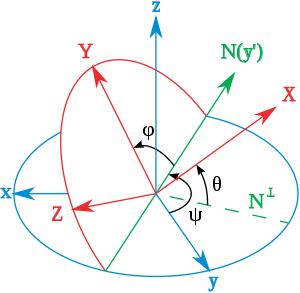
\includegraphics[width=0.4\textwidth]{figures/brian.png}
\caption{Euler angles}
\label{fig:euler}
\end{figure}

\subsection{Formulation}
Even though we are not measuring yaw ($\psi$), we still take it to acount in the system states since it does have an impact in giroscopic measures. The system state is defined in equation \ref{eq:system}

\begin{equation}
    \label{eq:system}
    x_k = 
        \begin{pmatrix}
            \varphi_k \\
            \theta_k \\
            \psi_k
        \end{pmatrix}
\end{equation}

The accelerometer measurements will be transformed to attitude measurements through a simple transformation defined in equation \ref{eq:meas}. It is simply the angles in two directions of the gravity vector with the $xy$ plane of the sensor.

\begin{equation}
    \label{eq:meas}
    z =
    \begin{pmatrix}
        \theta\\
        \varphi
    \end{pmatrix}
    = 
    \begin{pmatrix}
        asin \left( \frac{a_x}{g} \right) \\
        asin \left( -\frac{a_y}{g \cos \theta} \right)
    \end{pmatrix}
\end{equation}

Consequently, the expression of $H$ following equation \ref{eq:non_linear_meas} is very simple, and is defined in equation \ref{eq:H}

\begin{equation}
\label{eq:H}
H =
\begin{pmatrix}
1 & 0 & 0 \\
0 & 1 & 0
\end{pmatrix}
\end{equation}

To complete the formulation, we need to relate the angular rates measured by the gyroscope with the system state.
We need a transformation between the angular rates from gyroscope and the angular velocities of the fixed frame.

In \cite{ekf} it is described transformation defined in equation \ref{eq:euler_transf}. To obtain the transformation from gyroscope angular rates to euler angle velocities, we just need to invert the matrix from equation \ref{eq:euler_transf} and obtain the one in equation \ref{eq:T}.

To clarify the notation used in equations \ref{eq:euler_transf} and \ref{eq:T}:
\begin{itemize}
\item $\dot{\varphi}$, $\dot{\theta}$ and $\dot{\psi}$ are the angular velocities of the fixed frame
\item $p$, $q$ and $r$ are the angular rates from the gyroscopes.
\end{itemize}

\begin{equation}
    \label{eq:euler_transf}
    \begin{pmatrix}
        p \\
        q \\
        r
    \end{pmatrix}
    = \begin{pmatrix}
        1 & 0 & -\sin \theta \\
        0 & \cos \varphi & \sin \varphi \cos \theta \\
        -\sin \varphi & 0 & \cos \varphi \cos \theta
    \end{pmatrix}
    \begin{pmatrix}
        \dot{\varphi} \\
        \dot{\theta} \\
        \dot{\psi}
    \end{pmatrix}
\end{equation} 

\begin{equation}
    \label{eq:T}
    \dot{x} =
    \begin{pmatrix}
        \dot{\varphi} \\
        \dot{\theta} \\
        \dot{\psi}
    \end{pmatrix}
    = \begin{pmatrix}
        1 & \sin \varphi \tan \theta & \cos \varphi \tan \theta \\
        0 & \cos \varphi & - \sin \varphi \\
        0 & \frac{\sin \varphi}{\cos \theta}  & \frac{\cos \varphi}{\cos \theta}
    \end{pmatrix}
    \begin{pmatrix}
        p \\
        q \\
        r
    \end{pmatrix}
\end{equation} 

At this point, the update function can be defined as in equation \ref{eq:update}, which is just the previous state plus the state variation during a time step.

\begin{equation}
\label{eq:update}
f(x,p,q,r,dt) = x + T
\begin{pmatrix}
p \\ q \\ r
\end{pmatrix}
dt = x + \dot{x} dt
\end{equation}

Finally, the differencial matrix of $f$ looks very complicated (equation \ref{eq:F}) , but it is just computed taking the derivatives of $f$ with respect to the euler angles (not the angle rates from the sensors).

\begin{equation}
    \label{eq:F}
   F = I + dt
   \begin{pmatrix}
       q \cos\varphi \tan\theta - r \sin\varphi \tan \theta &
       q \sin \varphi \sec^2 \theta + r \cos \varphi \sec^2 \theta &
       0 \\
       -q \sin \varphi - r \cos \varphi
       & 0 & 0 \\
       q \cos \varphi \sec \theta - r \sin \varphi \sec \theta &
       q \sin \varphi \sec \theta \tan \theta + r \cos\varphi \sec \theta \tan  \theta &
       0
   \end{pmatrix}
\end{equation}


\subsection{Extended Kalman Filter}
Just as a reminder, the steps to perform the Extended Kalman Filter are depicted in equation \ref{eq:ekf}, for our defined system, and covariance matrices Q and R.
\begin{equation}
\label{eq:ekf}
\begin{array}{c}
    \hat{x}_k = f(x_{k-1},p,q,r,dt) \\
    \hat{P_k} = F_k P F_k' + Q \\
    K_k = \hat{P_k} H \left(H \hat{P_k} H' + R\right)^{-1} \\
    x_k = \hat{x}_k + K_k \left(z_k - H \hat{x}_k \right) \\
    P_k = \hat{P}_k - K H \hat{P}_k 
\end{array}
\end{equation}

The code used to compute the output of the Extended Kalman Filter has been implemented following the explanations from \cite{kim2011kalman} and can be found in \cite{repo}.